%%%%%%%%%%%%%%%%%%%%%%%%%%%%%%%%%%%%%%%%%
% a0poster Landscape Poster
% LaTeX Template
% Version 1.0 (22/06/13)
%
% The a0poster class was created by:
% Gerlinde Kettl and Matthias Weiser (tex@kettl.de)
% 
% This template has been downloaded from:
% http://www.LaTeXTemplates.com
%
% License:
% CC BY-NC-SA 3.0 (http://creativecommons.org/licenses/by-nc-sa/3.0/)
%
%%%%%%%%%%%%%%%%%%%%%%%%%%%%%%%%%%%%%%%%%

%----------------------------------------------------------------------------------------
%	PACKAGES AND OTHER DOCUMENT CONFIGURATIONS
%----------------------------------------------------------------------------------------

\documentclass[a0,landscape]{a0poster}

\usepackage{multicol} % This is so we can have multiple columns of text side-by-side
\columnsep=100pt % This is the amount of white space between the columns in the poster
\columnseprule=3pt % This is the thickness of the black line between the columns in the poster

\usepackage[svgnames]{xcolor} % Specify colors by their 'svgnames', for a full list of all colors available see here: http://www.latextemplates.com/svgnames-colors

\usepackage{times} % Use the times font
%\usepackage{palatino} % Uncomment to use the Palatino font

\usepackage{graphicx} % Required for including images
\graphicspath{{figures/}} % Location of the graphics files
\usepackage{booktabs} % Top and bottom rules for table
\usepackage[font=small,labelfont=bf]{caption} % Required for specifying captions to tables and figures
\usepackage{amsfonts, amsmath, amsthm, amssymb} % For math fonts, symbols and environments
\usepackage{wrapfig} % Allows wrapping text around tables and figures
 \usepackage{float}
 \usepackage{hyperref}
\begin{document}

%----------------------------------------------------------------------------------------
%	POSTER HEADER 
%----------------------------------------------------------------------------------------

% The header is divided into three boxes:
% The first is 55% wide and houses the title, subtitle, names and university/organization
% The second is 25% wide and houses contact information
% The third is 19% wide and houses a logo for your university/organization or a photo of you
% The widths of these boxes can be easily edited to accommodate your content as you see fit

\begin{minipage}[b]{0.55\linewidth}
\veryHuge \color{NavyBlue} \textbf{Honeypot Configuration and Data Analysis} \color{Black}\\ % Title
%\Huge\textit{Honeypot Configuration and Data Analysis}\\[1cm] % Subtitle
\huge \textbf{Jared Campbell \& David Zehden}\\ % Author(s)
\huge The University of Texas at Austin\\ % University/organization
\end{minipage}
%
%
%
\begin{minipage}[b]{0.19\linewidth}
%
\includegraphics[width=20cm]{logo.png} % Logo or a photo of you, adjust its dimensions here
\end{minipage}

\vspace{1cm} % A bit of extra whitespace between the header and poster content

%----------------------------------------------------------------------------------------

\begin{multicols}{3} % This is how many columns your poster will be broken into, a poster with many figures may benefit from less columns whereas a text-heavy poster benefits from more

%----------------------------------------------------------------------------------------
%	ABSTRACT
%----------------------------------------------------------------------------------------

\color{Black} % Navy color for the abstract

\section*{Abstract}

This project aims to build a honeypot server and analyze the data it collects. The goal of a honeypot server is to create vulnerable server on the open internet which we expect will be attacked by malicious actors. These attacks will be logged by the server, then we will analyze the data collected to find common trends in the attacks. Our honeypot will collect data on both an attacking machine and the attacks it directs at the honeypot. Our honeypot server is hosted on an Amazon Web Services (AWS) virtual server instance. The network for the server has been configured to allow all incoming traffic on monitored ports we expect to be targeted (such as SSH). We then analyzed the collected data using Python to find trends in attacker IP addresses, attacker operating systems, attacked ports, and timing of attacks. The honey pot was successful in collecting a large amount of attack data, averaging over 1000 unique data points per day. Our research has determined that a honeypot server is an effective tool for monitoring potential attacks on a network. We have also found honeypots to be highly configurable which allows for the collection of data specific to an organization's needs. 
%----------------------------------------------------------------------------------------
%	INTRODUCTION
%----------------------------------------------------------------------------------------

%\color{SaddleBrown} % SaddleBrown color for the introduction

\section*{Introduction}

A honeypot is a server that is made intentionally vulnerable in order to attract the attention of malicious actors. The server then logs any attempts by attackers to exploit and gain access to it. The goal is for researchers to be able to analyze common trends in the kinds of attacks used by malicious actors and even possibly discover new kinds of attacks that have never been seen before.  

While many different types of honeypot tools exist, we used Modern Honeypot Network (MHN) as the backbone of our project. MHN provides a nice interface for adding particular sensors and viewing data collected over a period of time. As seen in Figure 1.
\begin{figure}[H]
	\begin{center}
	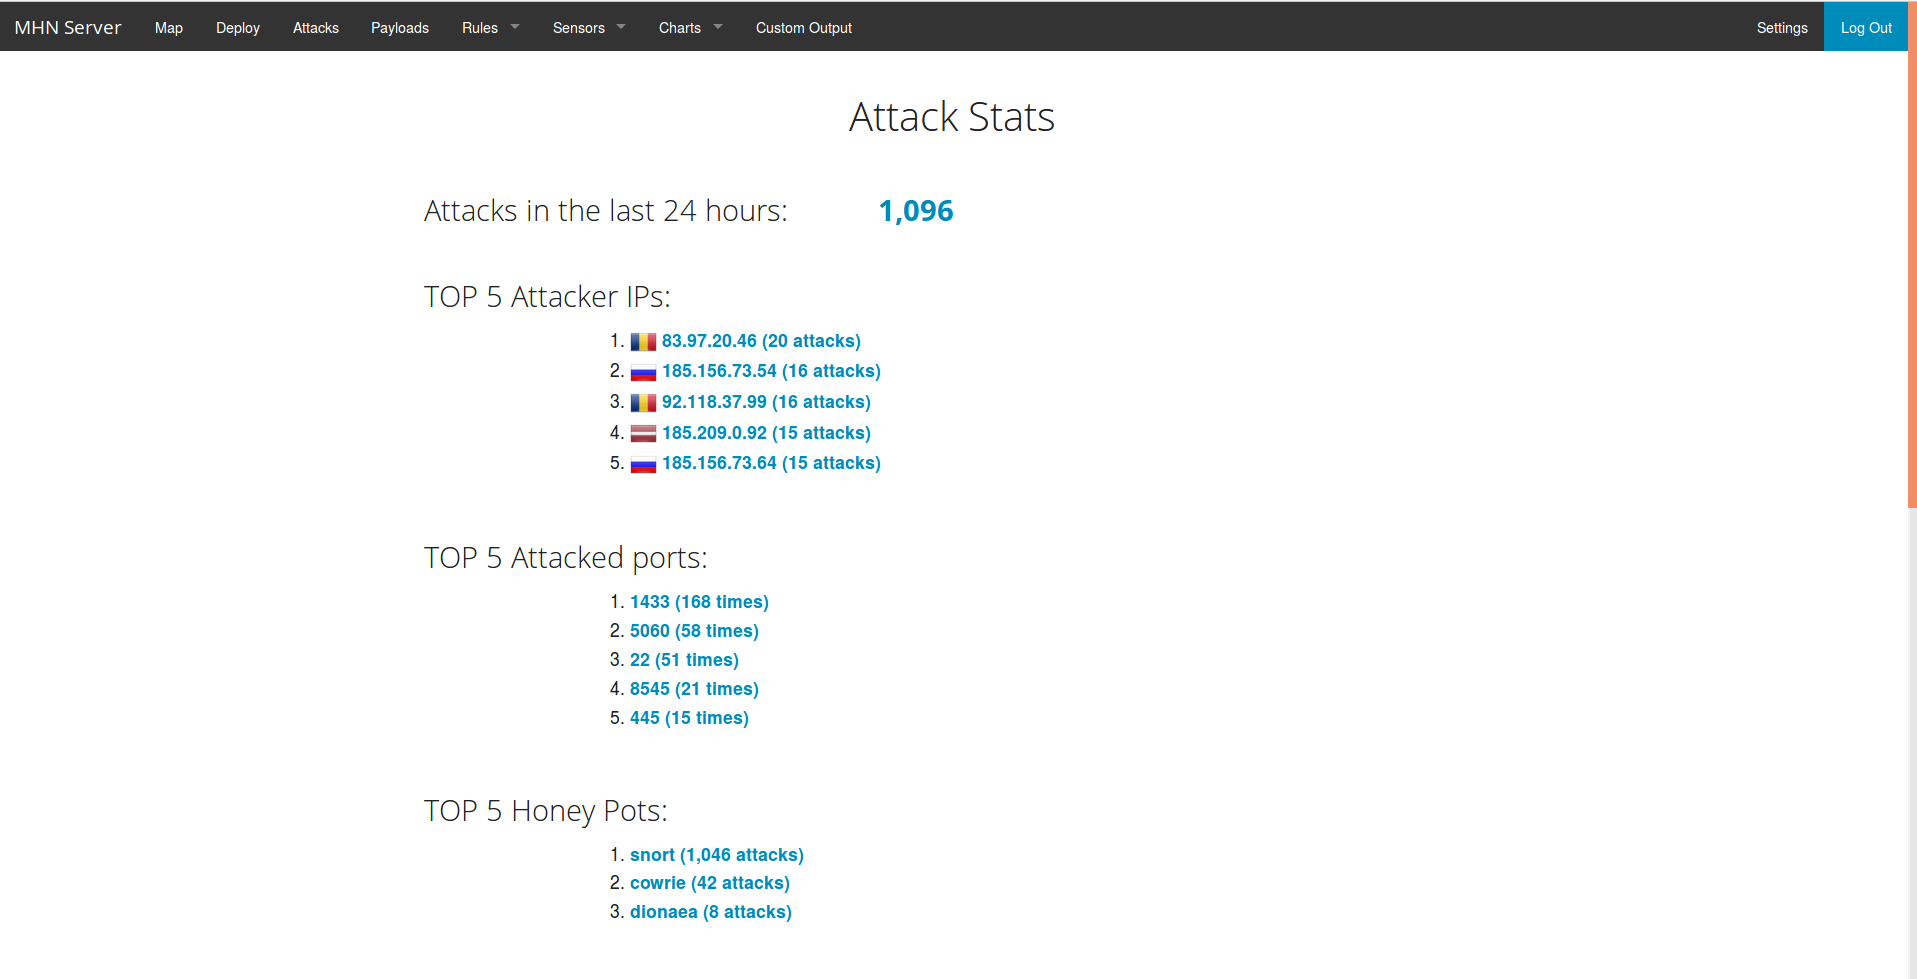
\includegraphics[width=28cm]{mhn.png}
	\caption{The Modern Honeypot Network Dashboard}
	\end{center}
\end{figure} 
%\begin{center}[H]
%	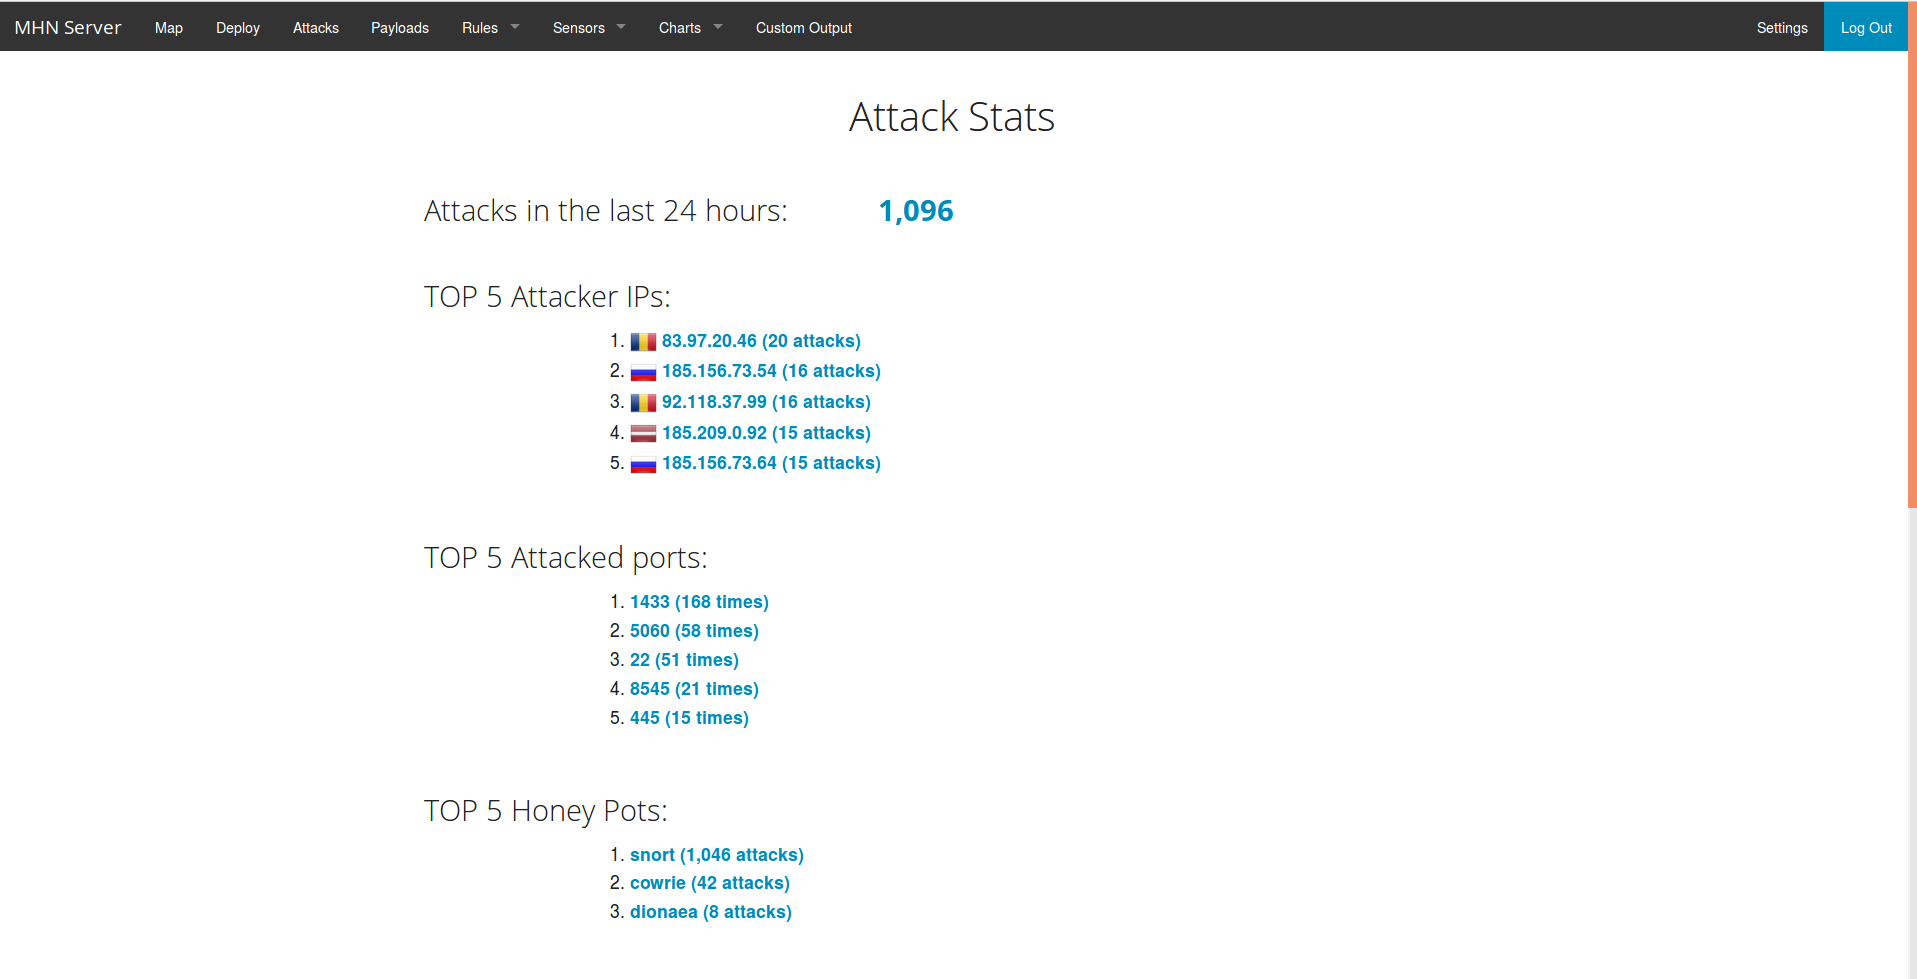
\includegraphics[width=20cm]{mhn.png} % Logo or a photo of you, adjust its dimensions here
	
%\end{center}
%----------------------------------------------------------------------------------------
%	OBJECTIVES
%----------------------------------------------------------------------------------------

\color{Black} % DarkSlateGray color for the rest of the content

\section*{Main Objectives}

\begin{enumerate}
\item Setup Amazon Web Services EC2 instance
\item Explore Honeypot options
\item Deploy Honeypot of choice on AWS
\item Configure Honeypot as needed
\item Collect data over time
\item Explore collected data to determine trends
\end{enumerate}

%----------------------------------------------------------------------------------------
%	MATERIALS AND METHODS
%----------------------------------------------------------------------------------------

\section*{Setup}
The three sensors used by the honeypot, Dionaea, Cowrie, and Snort, were each initially individually configured through MHN. We then manually configured the logging levels of each sensors to ensure relevant data was logged separately from error and debugging information so that it could be parsed by our Python analysis scripts. 

We have also configured the AWS server's firewall and security groups. We are allowing all inbound network traffic on all ports monitored by the honeypot (SSH, FTP, HTTP(S), etc.) and denying all outbound traffic. SSH access is restricted to our own SSH keys, and the SSH port has been changed from the default of 22 to allow Cowrie to monitor attacks on port 22. Password logins are denied and root login is also denied. 

For data analysis, we used the \texttt{mongoexport} command line tool to export data collected by MHN to JSON files. We used \texttt{SCP} to securely copy these files onto our local machines. Then we used Jupyter notebooks to explore data. Primarily, the \texttt{matplotlib}, \texttt{numpy}, and \texttt{pandas} libraries were used to aid the development of our findings. Additionally, we modified MHN to include a new webpage for particularly interesting findings. Such findings were generated from a daily \texttt{cron} job we set up on the server to run scripts that we developed locally.

\section*{Results}

Our honeypot made over 20,000 detections. We received traffic from all over the world, as you can see in Figure 2. In order to generate this map, we took all the IPs we detected and used the \href{https://github.com/pieqq/PyGeoIpMap}{PyGeoIpMap} library.
\begin{figure}[H]
	\begin{center}
		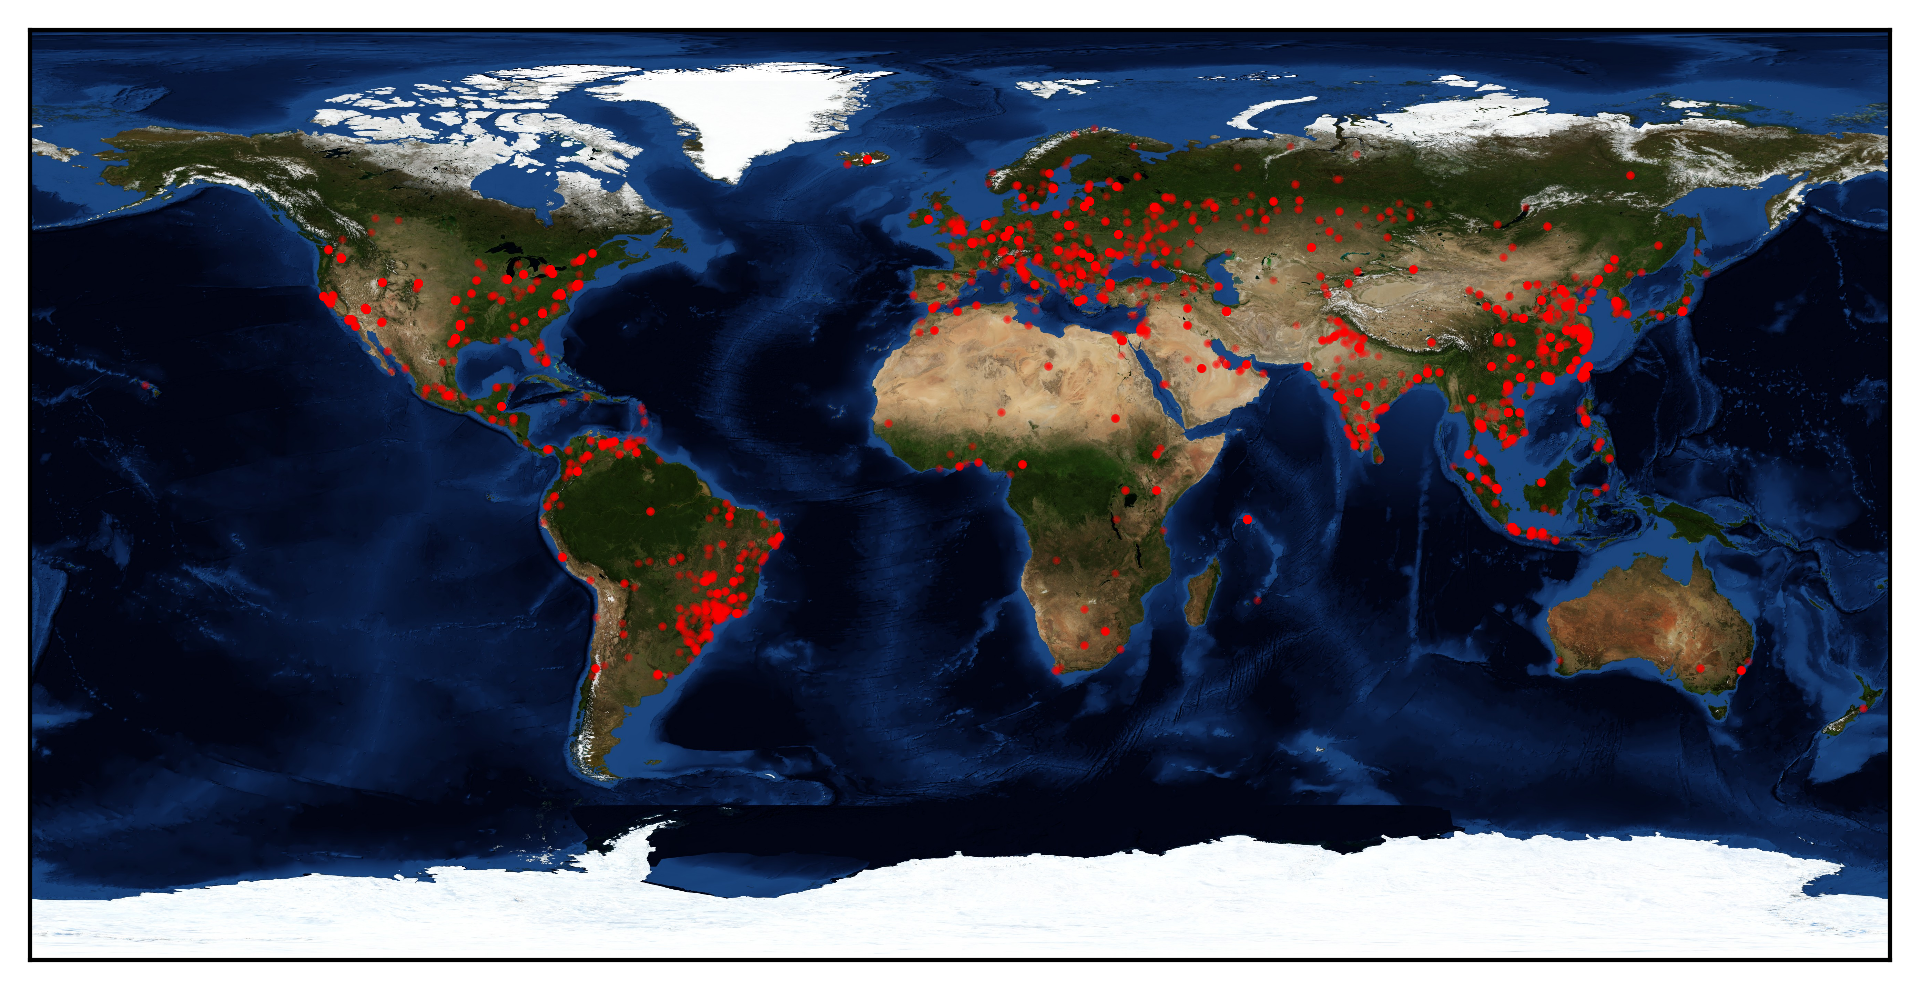
\includegraphics[width=30cm]{map.png}
		\caption{Approximate Locations of Detected IP Addresses}
	\end{center}
\end{figure} 

Additionally, we tried to break down the frequency with which we detected countries, as can be seen in Figure 3. 
\begin{figure}[H]
	\begin{center}
		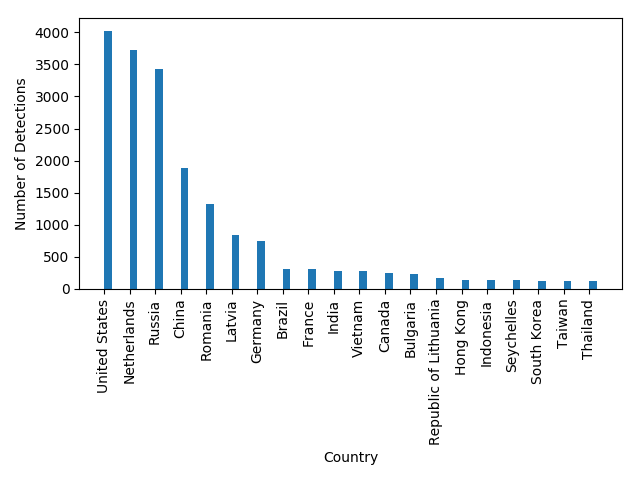
\includegraphics[width=25cm]{top_countries.png}
		\caption{Breakdown of Detections by Country}
	\end{center}
\end{figure} 

We also broke down our detections by time of day, as seen in Figure 4.

\begin{figure}[H]
	\begin{center}
		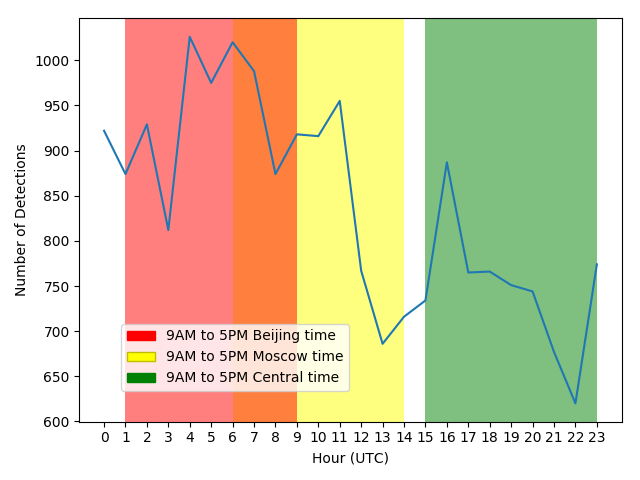
\includegraphics[width=25cm]{time_breakdown.png}
		\caption{Breakdown of Detections by Time of Day (UTC)}
	\end{center}
\end{figure} 

Finally, we observed the types of operating systems that our "attackers" were using.
\begin{figure}[H]
	\begin{center}
		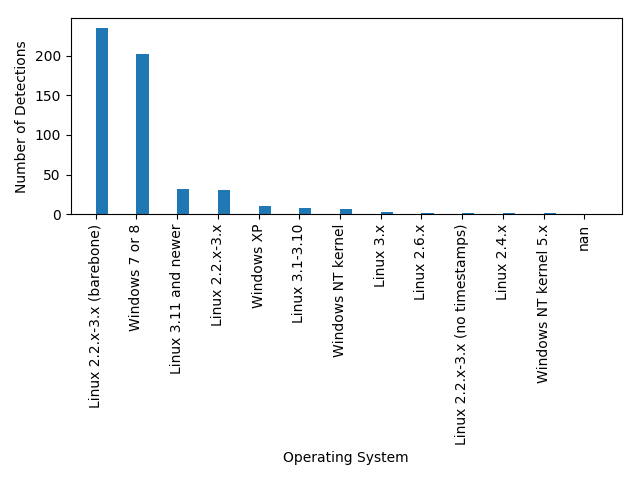
\includegraphics[width=25cm]{top_os.png}
		\caption{Breakdown of Detected Operating Systems}
	\end{center}
\end{figure} 


%------------------------------------------------
%----------------------------------------------------------------------------------------
%	RESULTS 
%----------------------------------------------------------------------------------------

\section*{Conclusion}
In order to research the effectiveness of honeypots, we implemented and configured our own honeypot on an AWS server. Our honeypot network collected even more data than we expected over the course of a single week. We have analyzed the data collected by our honeypot network to find trends in the origin of attacks, the hardware used for attacks, which services are most heavily targeted, and more. 

We have also seen that different honeypot solutions offer both various types of data and different quantities of data. From our findings, we could see that Snort was was able to capture a massive volume of information, but it was data that was generally more surface level. In contrast, Dionaea could provide examples of malware binaries that attackers attempted to run. However, this happened very infrequently, so it ultimately did not provide a great deal of data.

Our research has demonstrated that honeypots are an effective tool for monitoring malicious activity on a network. Our research also shows that honeypots can collect large amounts of data on many different types of trends. The data collected by a honeypot can be tailored to suit any organizations specific needs, making honeypots an effective tool not only for research, but also for securing enterprise environments. 

%----------------------------------------------------------------------------------------

\end{multicols}
\end{document}
